
 \begin{figure}[h!]
 \begin{center}
 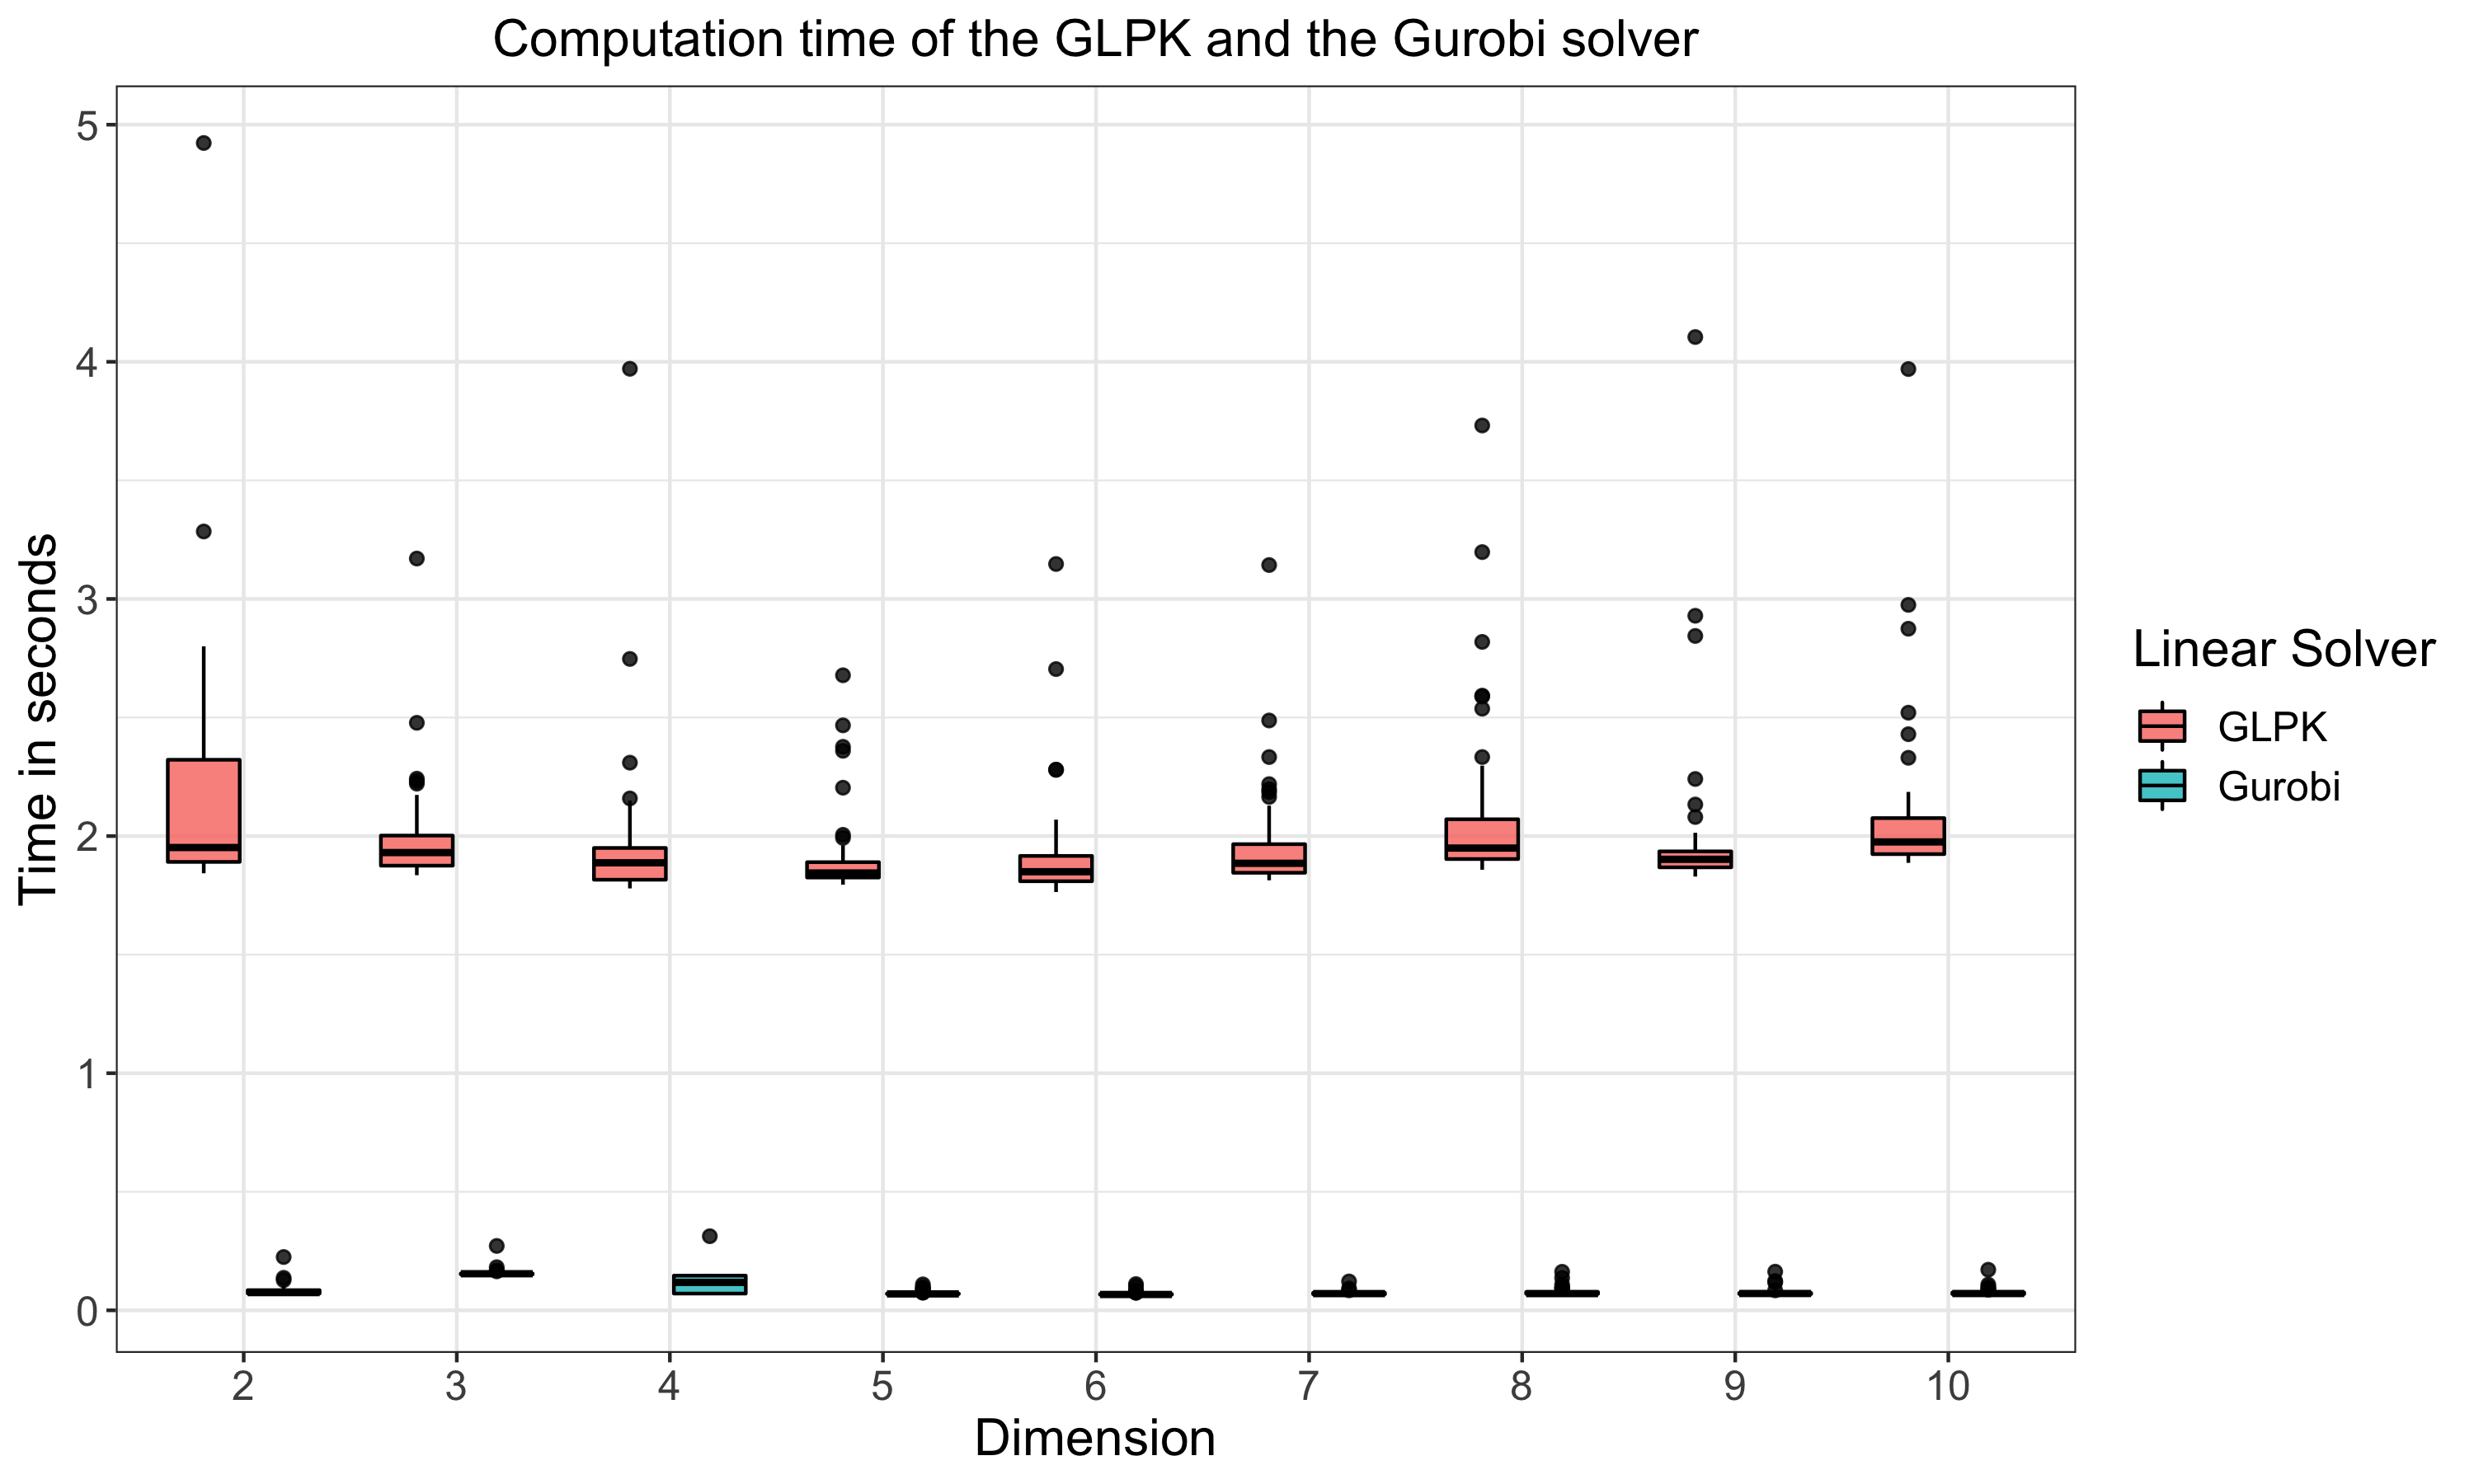
\includegraphics[width=1\textwidth]{boxplots_glpk_gurobi.jpg}% This is a *.eps file
 \end{center}
 \caption{Computation time of the GLPK linear solver (red) and the Gurobi linear solver (green) to solve the uniform/length-weighted edge-loss minimal problems in Algorithm 1. We perform experiments on $90$ data sets, 10 for each dimension 2-10, generated from the normal distribution. The horizontal axis is the dimension of the data set, and the vertical axis is the time it takes to solve an optimization problem. We observe that the Gurobi solver is consistently faster than the GLPK solver and that computation time seems fairly constant across dimension.}\label{fig:glpk_gurobi}
 \end{figure}

% % \begin{figure}[h!]
% % \begin{center}
% % 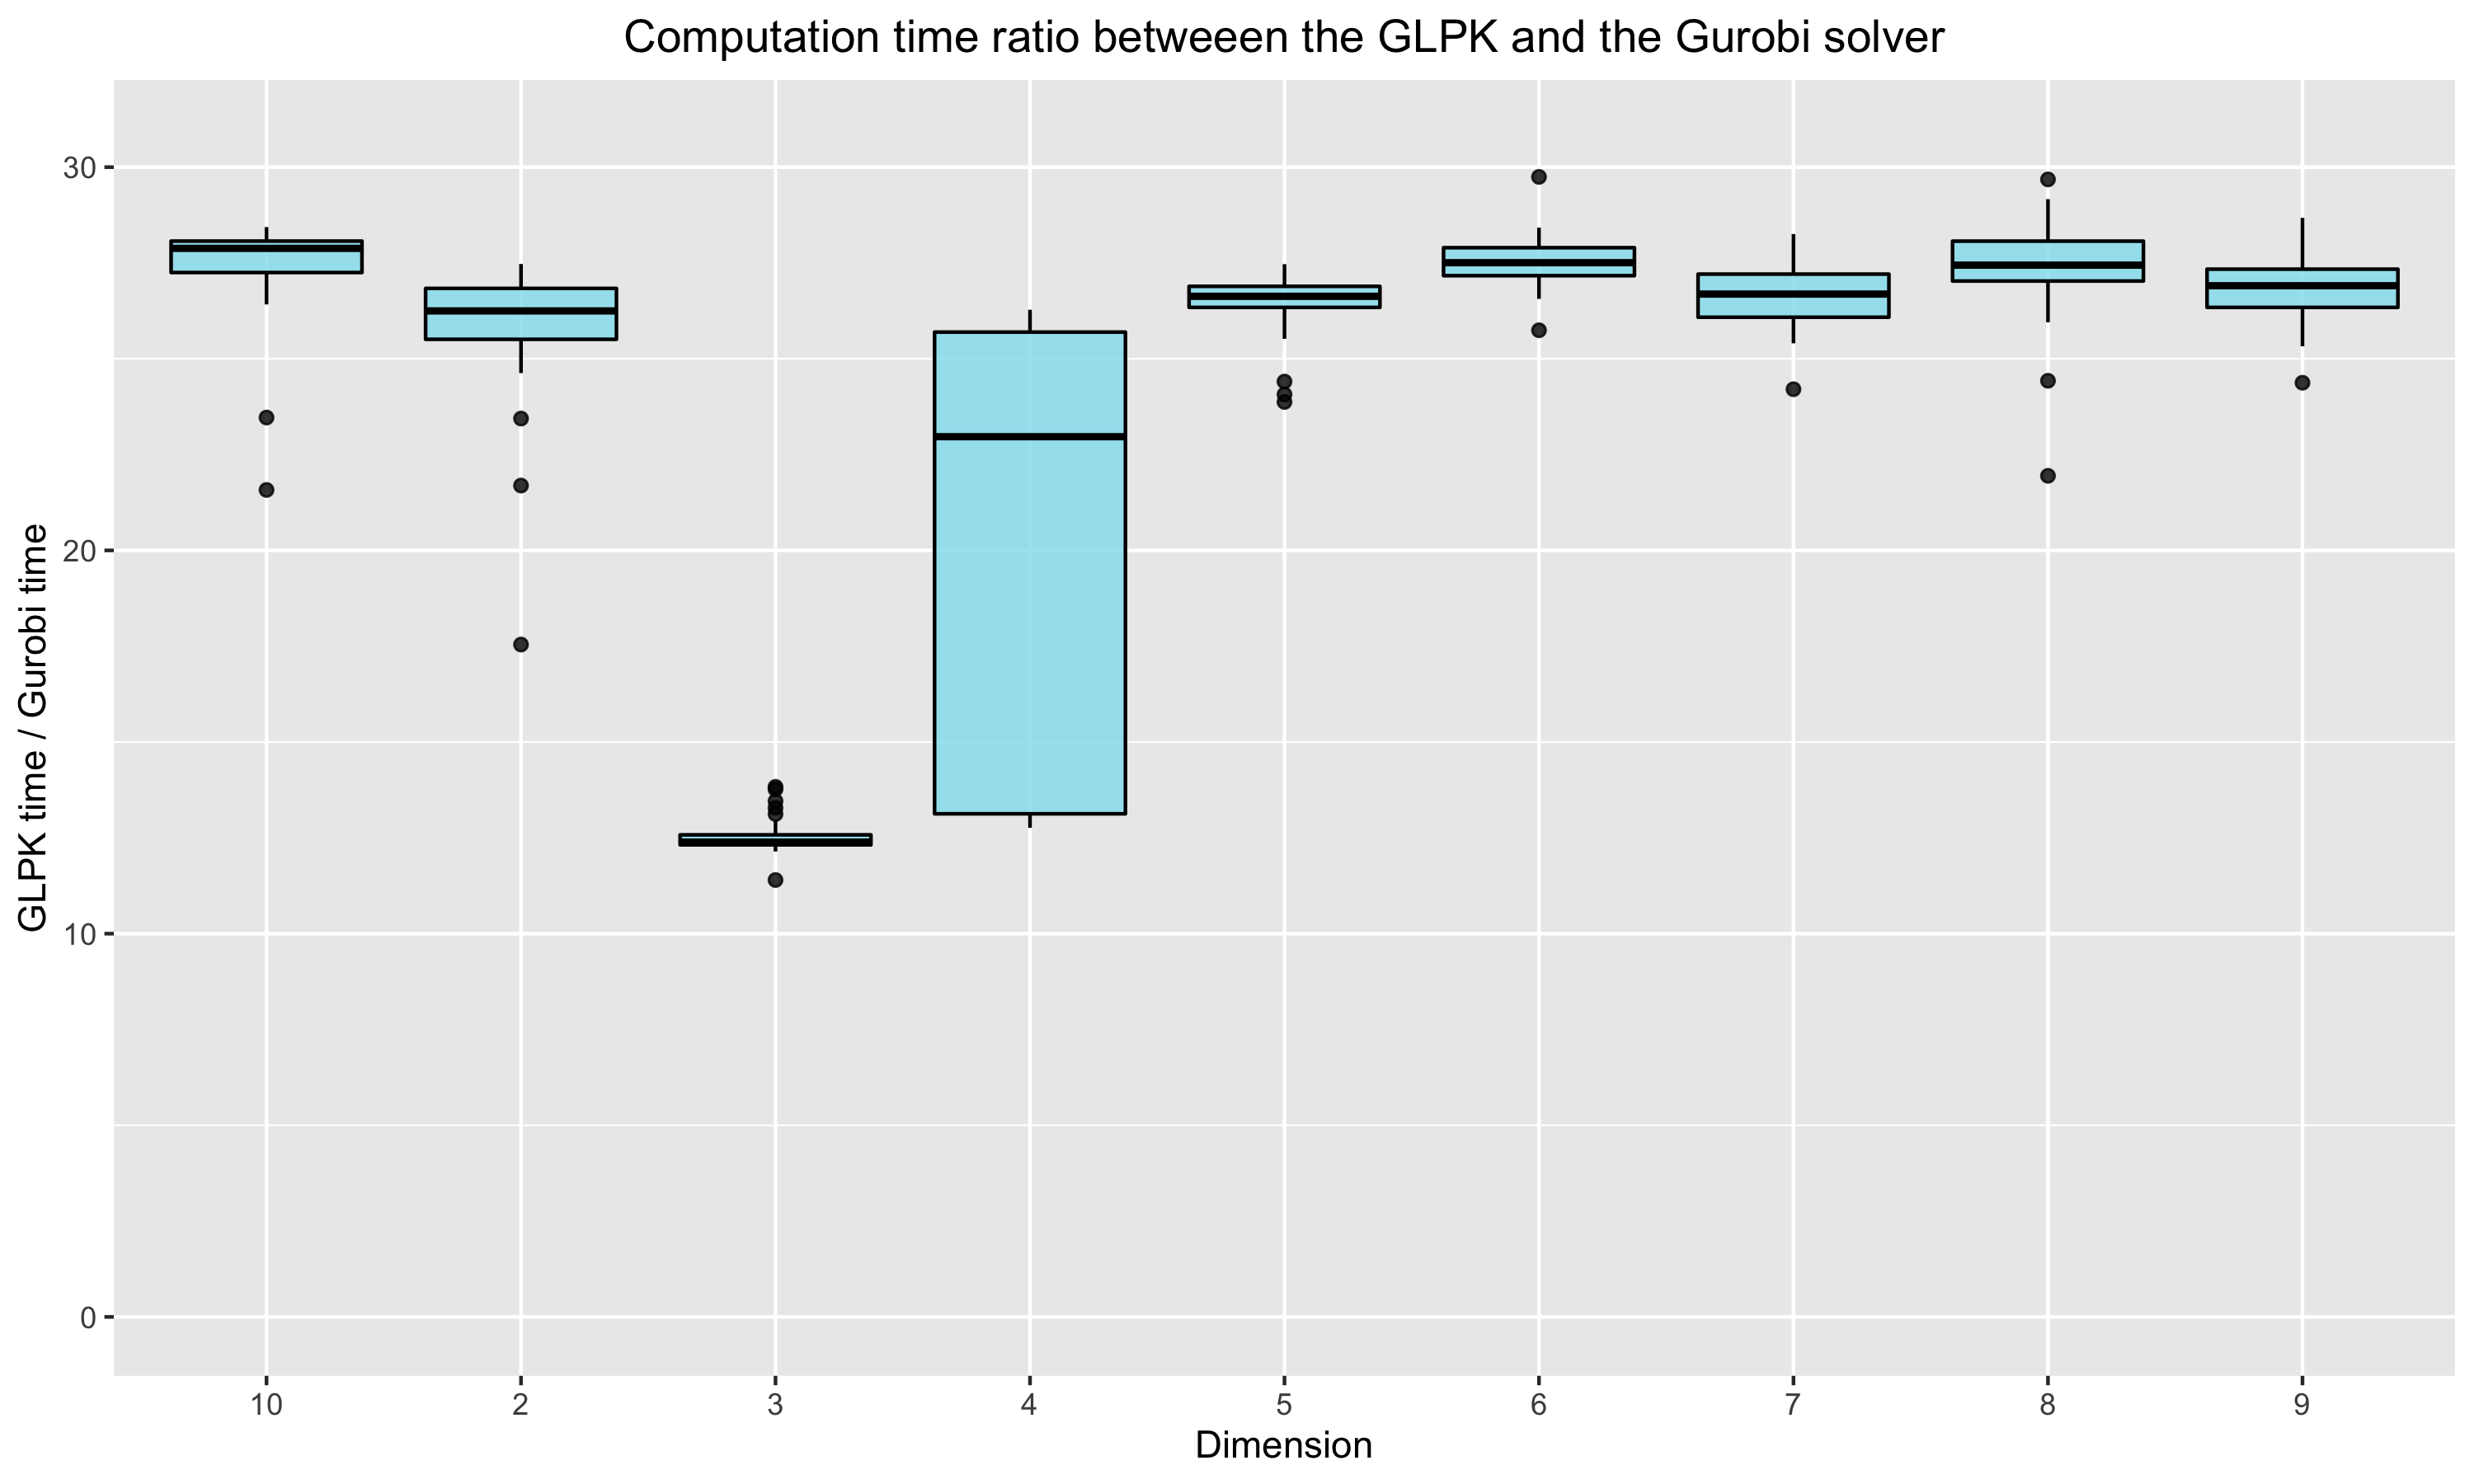
\includegraphics[width=1\textwidth]{figures/computationratio_glpk_gurobi.png}% This is a *.eps file
% % \end{center}
% % \caption{Computation time ratio of the GLPK and Gurobi linear solver. We observe that the Gurobi solver can be a lot faster than the GLPK solver.}\label{fig:glpk_gurobi}
% % \end{figure}
